\chapter{Model-Experiment Comparison}\label{c:compare}

In this chapter we'll discuss some general methods for comparing model predictions with experimental observations.  We are interested in being able to answer the questions, \emph{How good is the model?}, or more specifically, \emph{How good is the model at predicted the behavior of the physical system?}  We'll also present examples that show how these general concepts can be applied to particular models and experiments such as static and first-order models of physical systems like bending beams and temperature sensors.

We can make both \glspl{qualitative comparison} and \glspl{quantitative comparison} between model predictions and experimental data.  A qualitative comparison is based on subjective criteria such as does the time-response of our model ``look like'' the observed experimental data.  Qualitative evaluation is important, but it can only get us so far. As engineers we'll want to quantify our evaluation to put the comparison in subjective, numerical terms (hopefully with units!).  


\section{Quantitative Comparison}

\renewcommand{\ThisFigWidth}{0.3}
\begin{figure}[th!]
\centering
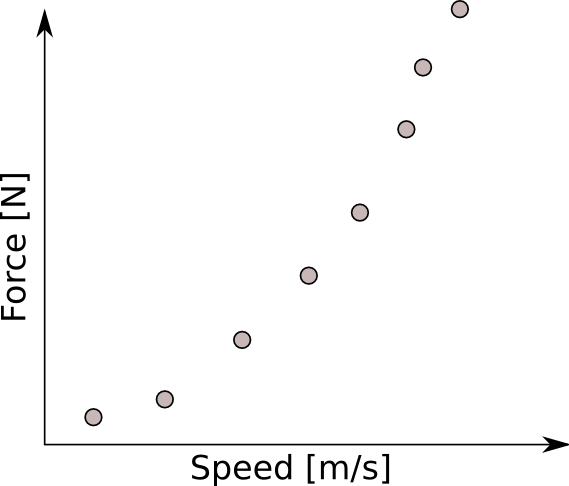
\includegraphics[width=\ThisFigWidth\textwidth]{model_fit_data.png}
\caption{Graph of our empirical measurements of pulling something through some fluid and measuring the drag force.  The individual data points are shown as circles.}
\label{f:modeldata}
\end{figure}

Let's consider an example.  Imagine we are measuring the drag force on something (a boat, surfboard, fish, diver, hang glider, etc.) as it moves through a fluid (air, water, mercury, etc.).  We pull our thing through our fluid at a few different speeds and measure the force.  If we plot our data it might look something like Figure~\ref{f:modeldata}.  Now that we have data, we might consider what type of (mathematical) model would be a good representation (or fit) to the model.  One thing we might try is to consider a \emph{linear model}, i.e., we are proposing that there is linear realtionship between speed and drag force.  To be more specific, we are proposing that the function $F_{\mathrm{drag}}=m(V)$ could be a ``good'' representation of our observation.
\begin{figure}[hb!]
\centering
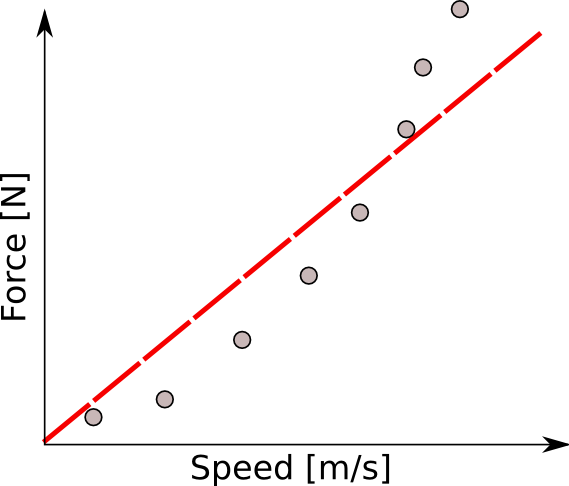
\includegraphics[width=\ThisFigWidth\textwidth]{model_fit_line.png}
\caption{Graph of our empirical measurements with a notional linear model.  The data (circles) and the linear model (red dashed line) are shown together.}
\label{f:modelline}
\end{figure}
Based on our data and our proposed model we could then come up with a value for the $m$ term in our model.  Figure~\ref{f:modelline} illustrates what this might look like.  Qualitatively this model ``looks pretty good'', but...

Alternatively, we might consider a different model.  Perhaps we could try a \emph{quadratic model} of the form $F_{\mathrm{drag}}=c(V^2)$.  Again, there is just one parameter in our model ($c$) that we'll need to choose so that the model and the data are similar. If we can find a reasonable quadratic coefficient we might get something that looks like Figure~\ref{f:modelquad}.  Based on this graph we could conclude, qualitatively, that the quadratic model is a ``better fit'' than the linear model.  We could also conclude that the error between the quadratic model and the data is ``small'', but we can't really get beyond these qualitative explanations.

\begin{figure}[bh!]
\centering
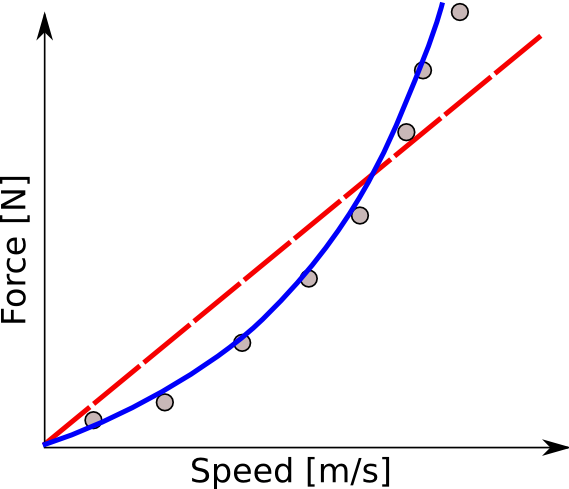
\includegraphics[width=\ThisFigWidth\textwidth]{model_fit_quad.png}
\caption{Graph of our empirical measurements with a notional linear and quadratic models.  The data (circles), linear model (red dashed line) and quadratic model (solid blue line) are shown together.}
\label{f:modelquad}
\end{figure}

\section{Square Error}

Residual
\[
r_i = y_i - \hat{y}_i
\]
